\documentclass[usenames,dvipsnames]{beamer}
% \documentclass[usenames,dvipsnames,handout]{beamer}


\usetheme{AnnArbor}
\usecolortheme{beaver}
\usecolortheme{dolphin}



\usepackage{commands}
\usepackage{faktor}
\usepackage{xfrac} 
\usepackage{amssymb}
\usepackage{stmaryrd}

\DeclareMathOperator{\AV}{AV}
\DeclareMathOperator{\Mat}{Mat}
\DeclareMathOperator{\Pol}{Pol}

\newcommand{\AVord}[1]{\AV^{\text{ord}}({#1})}
\newcommand{\Modord}[1]{\cM^{\text{ord}}({#1})}

\newcommand{\red}[1]{\textcolor{red}{#1}}
\newcommand{\blue}[1]{\textcolor{blue}{#1}}
\newcommand{\green}[1]{\textcolor{ForestGreen}{#1}}
\renewcommand{\char}{char}

%AUTHOR DETAILS
%%%%%%%%%%%%%%%%%%%%%%%%%%%%%%%%%%%%%%%%%%%%%%%%
\title[]{Isomorphism classes of abelian varieties over finite fields}
\subtitle{}
\author[Marseglia Stefano]{Marseglia Stefano}
\institute[]{Utrecht University}
\date{ICERM - January 31, 2019}

\begin{document}

\begin{frame}
\titlepage
\end{frame}

\begin{frame}{ Plan for today }
\begin{enumerate}[(a)]
 \pause \item equivalence of categories
       \begin{itemize}
        \item Deligne (ordinary over $\F_q$)
        \item Centeleghe-Stix (over $\F_p$ away from real primes)
       \end{itemize}
 \pause \item isomorphism classes of AV
       \begin{itemize}
        \item square-free case : ideal class monoid
        \item power of a sq-free : only Bass orders
       \end{itemize}
 \pause \item polarizations
       \begin{itemize}
        \item square-free ordinary case : working algorithm
        \item square-free Centeleghe-Stix case : working algorithm (conjectural)
        \item power of a sq-free : no algorithm :(
       \end{itemize}
 \pause \item bottle-necks
       \begin{itemize}
        \item over-orders (Tommy Hofmann?)
        \item weak eq. classes (I have a conjecture)
        \item CM-type (need to compute a splitting field)
        	\item polarizations (it should be possible to spread them)
       \end{itemize}
\end{enumerate}
\end{frame}

\begin{frame}{ Deligne's equivalence }
\begin{theorem}[Deligne '69]
Let $q=p^r$, with $p$ a prime. There is an equivalence of categories:
\[\begin{array}{cc}
\set{\text{\green{Ordinary} abelian varieties over $\F_q$}}	& A \\
\pause \updownarrow							& \downmapsto \\
\set{\parbox[p]{19em}{pairs $(T,F)$, where $T\simeq_\Z \Z^{2g}$ and $T\overset{F}{\to} T$ s.t.\\
- $F\otimes \Q$ is semisimple\\
- the roots of $\Char_{F\otimes\Q}(x)$ have abs. value $\sqrt{q}$\\
- \green{half of them are $p$-adic units}\\
- $\exists V:T\to T$ such that $FV=VF=q$
}}	& (T(A),F(A))
\end{array}\]
\end{theorem}
\pause
\begin{remark}
\begin{itemize}
 \item If $\dim(A)=g$ then $\rk(T(A))=2g$;
 \item $\Frob(A)\rightsquigarrow F(A)$.
\end{itemize}
\end{remark}
\end{frame}

\begin{frame}{ Centeleghe-Stix' equivalence }
\begin{theorem}[Centeleghe-Stix '15]
Let $p$ be a prime. There is an equivalence of categories:
\[\begin{array}{cc}
\set{\text{abelian varieties over \red{$\F_p$} \green{away from real primes}}}	& A \\
\pause \updownarrow							& \downmapsto \\
\set{\parbox[p]{19em}{pairs $(T,F)$, where $T\simeq_\Z \Z^{2g}$ and $T\overset{F}{\to} T$ s.t.\\
- $F\otimes \Q$ is semisimple\\
- the roots of $\Char_{F\otimes\Q}(x)$ have abs. value \red{$\sqrt{p}$}\\
- \green{$\Char_{F\otimes\Q}(\sqrt{p}) \neq 0$}\\
- $\exists V:T\to T$ such that $FV=VF=\red{p}$
}}	& (T(A),F(A))
\end{array}\]
\end{theorem}
\pause
\begin{remark}
\begin{itemize}
 \item If $\dim(A)=g$ then $\rk(T(A))=2g$;
 \item $\Frob(A)\rightsquigarrow F(A)$.
\end{itemize}
\end{remark}
\end{frame}

\begin{frame}{ equivalences in the square-free case}
Let $h$ be a square-free characteristic $q$-Weil polynomial.

Assume that $h$ is \textbf{ordinary} or, $q=p$ and $\bf{h(\sqrt{p})\neq 0}$.

\[\rightsquigarrow \text{an isogeny class $\cC_h$ (by Honda-Tate)}.\]
\pause Put
\begin{align*}
 K &:= \Q[x]/(h)\\
 F &:= x \mod (h)\\
 R &:= \Z[F,q/F] \subset K
\end{align*}
\pause We get:
% \vspace{-2 em}
\begin{theorem}[M.]
\[ \text{an equivalence } \cC_h \longleftrightarrow \set{ \text{fractional $R$-ideals } } \]
\[ \text{and } \faktor{\cC_h}{\simeq} \longleftrightarrow \faktor{\set{ \text{fractional $R$-ideals } }}{\simeq_R} \textcolor{blue}{=:\ICM(R) \text{ ideal class monoid}} \]

\end{theorem}
\end{frame}

\begin{frame}{ICM : Ideal Class Monoid}
Let $R$ be an order in a finite \'etale  $\Q$-algebra $K$.
% according to Bourbaki etale (over a field K) implies commutative and finite (since it is defined as being isomorphic to L^n for some extension L of K).
\begin{itemize}
   \pause \item Recall: for fractional $R$-ideals $I$ and $J$
    \[ I\simeq_R J \Longleftrightarrow \exists x \in K^\times \text{ s.t.~} xI=J \]
   \pause \item Define the \textbf{ideal class monoid} of $R$ as
    \[\ICM(R) := \faktor{\set{\text{fractional $R$-ideals}}}{\simeq_R}\]

   \pause \item We have
   \[ \ICM(R) \supseteq \Pic(R) \hspace{2.5 cm} \textcolor{blue}{\text{with equality iff $R=\cO_K$}} \]
   \pause \item ...and actually
   \[ \ICM(R) \supseteq \bigsqcup_{\scriptsize\parbox{5 em}{$R\subseteq S \subseteq \cO_K$\\over-orders}}\Pic(S) \qquad \textcolor{blue}{\text{with equality iff $R$ is Bass}} \]
\end{itemize}
\end{frame}

\begin{frame}{ simplify the problem  }
Study the isomorphism problem locally: (Dade, Taussky, Zassenhaus '62)
\begin{itemize}
\pause \item  \textbf{weak equivalence}:
\[I_\p\simeq_{R_\p} J_\p \text{ for every }\p\in \mSpec(R)\]
\pause \vspace{-6mm}\[\Updownarrow\]
\[1\in (I:J)(J:I)\quad \textcolor{blue}{\text{easy to check!}}\]
\pause \item Let $\cW(R)$ be the set of weak eq.~classes...\\
\pause ...whose representatives can be found in
	\[\set{\text{sub-$R$-modules of $\faktor{\cO_K}{\frf_R}$}}\quad \textcolor{blue}{\parbox{10 em}{finite! and most of the time not-too-big ...}}\]
\end{itemize}
\end{frame}

\begin{frame}{ Compute $\ICM(R)$ }
\pause Partition w.r.t. the multiplicator ring:
    \begin{columns}
    \begin{column}{0.5\textwidth}
      \[ \cW(R) = \bigsqcup_{R\subseteq S \subseteq \cO_K} \overline \cW(S)\]
      \[\ICM(R) = \bigsqcup_{R\subseteq S \subseteq \cO_K} \overline \ICM(S)\]
    \end{column}
\pause
    \begin{column}{0.5\textwidth}  %%<--- here
	\begin{center}
	\textcolor{blue}{\parbox{10em}{the ``bar'' means ``only classes with multiplicator ring S''}} 
	\end{center}
    \end{column}
    \end{columns}
\pause
   \begin{theorem}[M.]
    For every over-order $S$ of $R$, $\Pic(S)$ acts freely on $\overline{\ICM(S)}$ and
    \[ \overline\cW(S) = \overline{\ICM(S)}/\Pic(S) \]
\pause Repeat for every $R\subseteq S \subseteq \cO_K$:
    \[ \rightsquigarrow \ICM(R).\]
   \end{theorem}
    \red{Bottleneck 1: we need to compute all over-orders!} (Tommy Hoffman ?)
\end{frame}

\begin{frame}{ More details about: $\overline\cW(S)$ }
    Let $T$ be the (smallest) over-order of $S$ such that $S^{t}T$ is \red{invertible} in $T$.
    \pause Let $I$ be a fractional ideal with $(I:I)=S$. 
    \pause Since $I\cdot I^{t}=S^{t}$, it follows that $IT$ si invertible in $T$ and hence we can assume that $IT=T$ (up to weak equivalence).
    
    \pause We get that
    \[ \frf \subset I \subset T, \]
    where $\frf=(S:T)$.
    \begin{prop}
    \pause We can find all representatives of $\overline\cW(S)$ in the quotient
    \[ \cQ_{S}=\faktor{T}{\frf} \]
    \end{prop}
    \pause \red{Bottleneck 2: $\cQ_{S}$ might be too big! I have a "conjecture"...but no a proof}
\end{frame}

\begin{frame}{ The case "power of a square-free"  }
    Consider $\cC_h$ for $h=g^r$ with $g$ a square-free $q$-Weil polynomial. 
    Assume that $g$ is \textbf{ordinary} or, $q=p$ and $\bf{g(\sqrt{p})\neq 0}$.

    \pause Put
    \begin{align*}
    K &:= \Q[x]/(\red{g})\\
    F &:= x \mod (\red{g})\\
    R &:= \Z[F,q/F] \subset K
    \end{align*}
    \pause We get:
    % \vspace{-2 em}
    \begin{theorem}[M.]
    We have an equivalence
    \[ \cC_h \longleftrightarrow \set{ \text{fin.~gen.~torsion-free $R$-modules $M$ s.t.~$M\otimes_R K\simeq K^r$} }\blue{=:\cB(g^r)} \]
    \end{theorem}
\end{frame}

\begin{frame}{ The category $\cB(g^r)$ }
Recall that an $R$-module $M$ is \textbf{torsion-free} if the canonical morphism
\[ M \to M\otimes_R K \]
is injective.

\pause We can think of modules $M\in \cB(g^r)$ as \textbf{embedded} in $K^r$.

\pause The category $\cB(g^r)$ becomes more \green{explicit} and \green{computable} under certain assumption on the order $R$.

An order $R$ is called \red{Bass} if one of the following equivalent conditions holds:
\begin{itemize}
 \pause \item every over-order $R\subseteq S \subseteq \cO_K$ is Gorenstein (i.e. $S^t$ is invertible in $S$).
 \pause \item every fractional $R$-ideal $I$ is invertible in $(I:I)$.
 \pause \item $\ICM(R) = \bigsqcup_{R\subseteq S\subseteq \cO_K} \Pic(S)$.
\end{itemize}
\end{frame}

\begin{frame}{ $\cB(g^r)$ in the Bass case }
\begin{thm}[Bass]
 Assume that $R$ is a Bass order.
 \pause Then for every $M\in \cB(g^r)$ there are fractional $R$-ideals $I_1,\ldots,I_r$ such that 
 \[ M \simeq_R I_1\oplus \ldots \oplus I_r. \qquad\green{\parbox{12em}{everything is a direct sum\\of fractional ideals}}\]
 \pause Moreover, given $M=\bigoplus_{k=1}^r I_k$ and $M'=\bigoplus_{k=1}^r J_k$ we have that 
 \[ M\simeq_R M' \Longleftrightarrow
 \begin{cases}
  (I_k:I_k)=(J_k:J_k) \text{ for every $k$, and } \\
  \prod_{k=1}^r I_k \simeq_R \prod_{k=1}^r J_k
 \end{cases}
 \pause \parbox{7em}{\green{generalization of Steinitz theory}}
 \]
\end{thm}
\end{frame}

\begin{frame}{ $\cB(g^r)$ in the Bass case }
\begin{corollary}
 Assume that $R$ is Bass. Then for every $M\in \cB(g^r)$ there are over orders $S_1\subseteq \ldots \subseteq S_r$ of $R$ and a fractional ideal $I$ invertible in $S_r$ such that
 \[ M\simeq S_1\oplus\ldots\oplus S_{r-1}\oplus I \]
\end{corollary}
  \pause We have a \green{simple description} of morphisms in $\cB(g^r)$.

  For example, for $M$ as above:
  \pause {\small
\[ \End_R(M) = 
    \begin{pmatrix}
    S_1 	& S_2 	   & \ldots & S_{r-1} & I \\
    (S_1:S_2) 	& S_2 	   & \ldots & S_{r-1} & I \\
    \vdots 	& \vdots   & \ddots & \vdots  & \vdots \\
    (S_1:S_{r-1}) 	& (S_2:S_{r-1})& \ldots & S_{r-1} & I \\
    (S_1:I) 	& (S_2:I)& \ldots & (S_{r-1}:I) & (I:I)
    \end{pmatrix}
    \]
}
and 
\pause 
\[\Aut_R(M)=\set{ A \in \End_R(M) \cap \GL_r(K) : A^{-1} \in \End_R(M) }.\]
\end{frame}


\begin{frame}{ Consequences for $\cC_h$ }
\begin{corollary}
Assume $R=\Z[F,q/F]$ is Bass.
Then
 \begin{itemize}
  \pause \item \ 
  \vspace{-1em}
  \[ \faktor{\cC_h}{ \simeq } \longleftrightarrow \set{ (S_1\subseteq S_2 \subseteq \ldots \subseteq S_r , [I]_{\simeq}) : \parbox{7em}{$R\subseteq S_1$,\\ $I$ a frac. $R$-ideal with $(I:I)=S_r$}  } \]
  \pause \item for every $A\in \cC_h$, say $A\sim B^r$ with $h_B=g$, there are 
  \vspace{-1em}
  \[C_1,\ldots,C_r \sim B \text{ such that } A \simeq C_1\times \ldots \times C_r \qquad\green{\parbox{8em}{everything\\ is a product}} \]
  \vspace{-1em}
  \pause \item if 
  \vspace{-1em}
  \[ A \longleftrightarrow \bigoplus_k I_k \text{ and } B \longleftrightarrow \bigoplus_k J_k \]
  \vspace{-1em}
  then 
  \vspace{-1em}
  \[ \mu \in \Hom(A,B) \longleftrightarrow \Lambda \in \Mat_{r\times r}(K) \text{ s.t. } \Lambda_{h,k}\in (J_h:I_k) \]
  \pause Moreover, $\mu$ is an \red{isogeny} if and only if $\det(\Lambda) \in K^\times$
 \end{itemize}
\end{corollary}
\end{frame}

% \begin{frame}{Example 1}
% \begin{figure}
%     \begin{columns}%
%         \begin{column}{0.4\textwidth}%
%             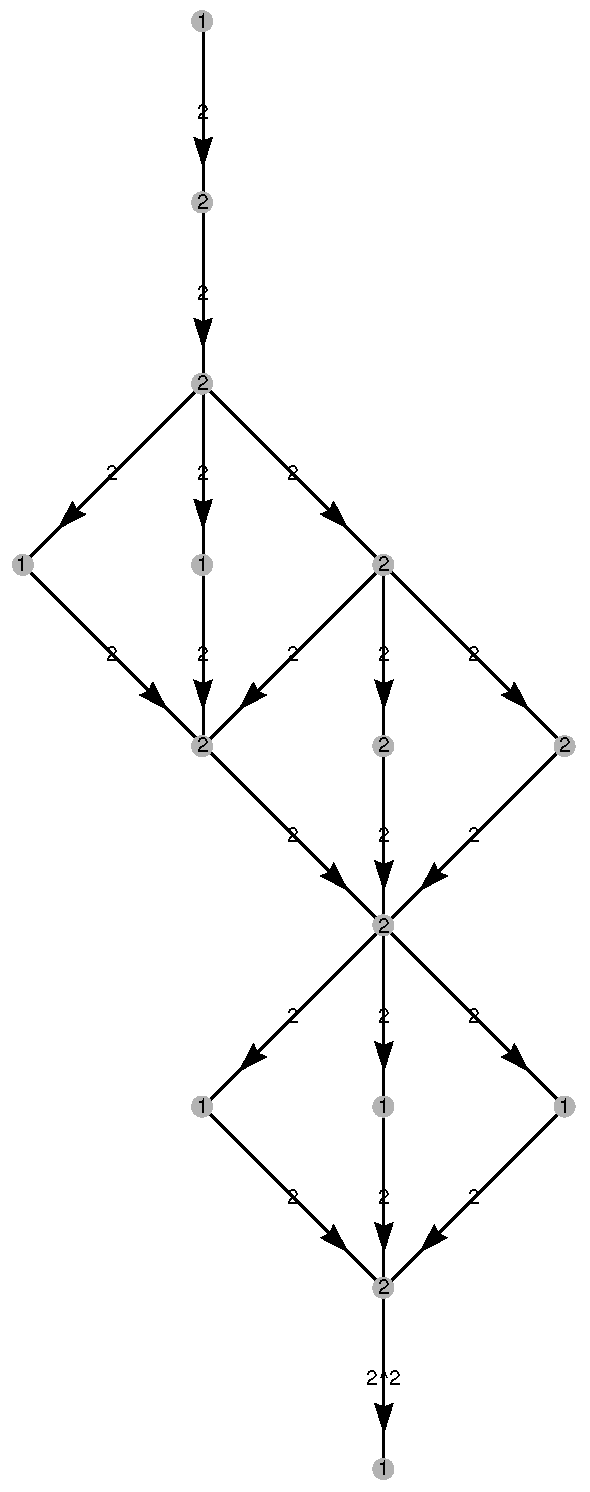
\includegraphics[width=0.65\textwidth]{graph-4}
%         \end{column}%
%         \begin{column}{0.6\textwidth}%
%             Weak equivalence classes of the monogenic order of $\Q[x]/(f)$ where $f=x^3+31x^2+43x+77$.\\
% 	    - vertices are orders, labeled by $\# \bWk$\\
% 	    - edges are inclusions, labeled by the index
%         \end{column}%
%     \end{columns}
% \end{figure}
% \end{frame}
% 
% \begin{frame}{Example 2}
% \vspace{-2 em}
% \begin{figure}
%     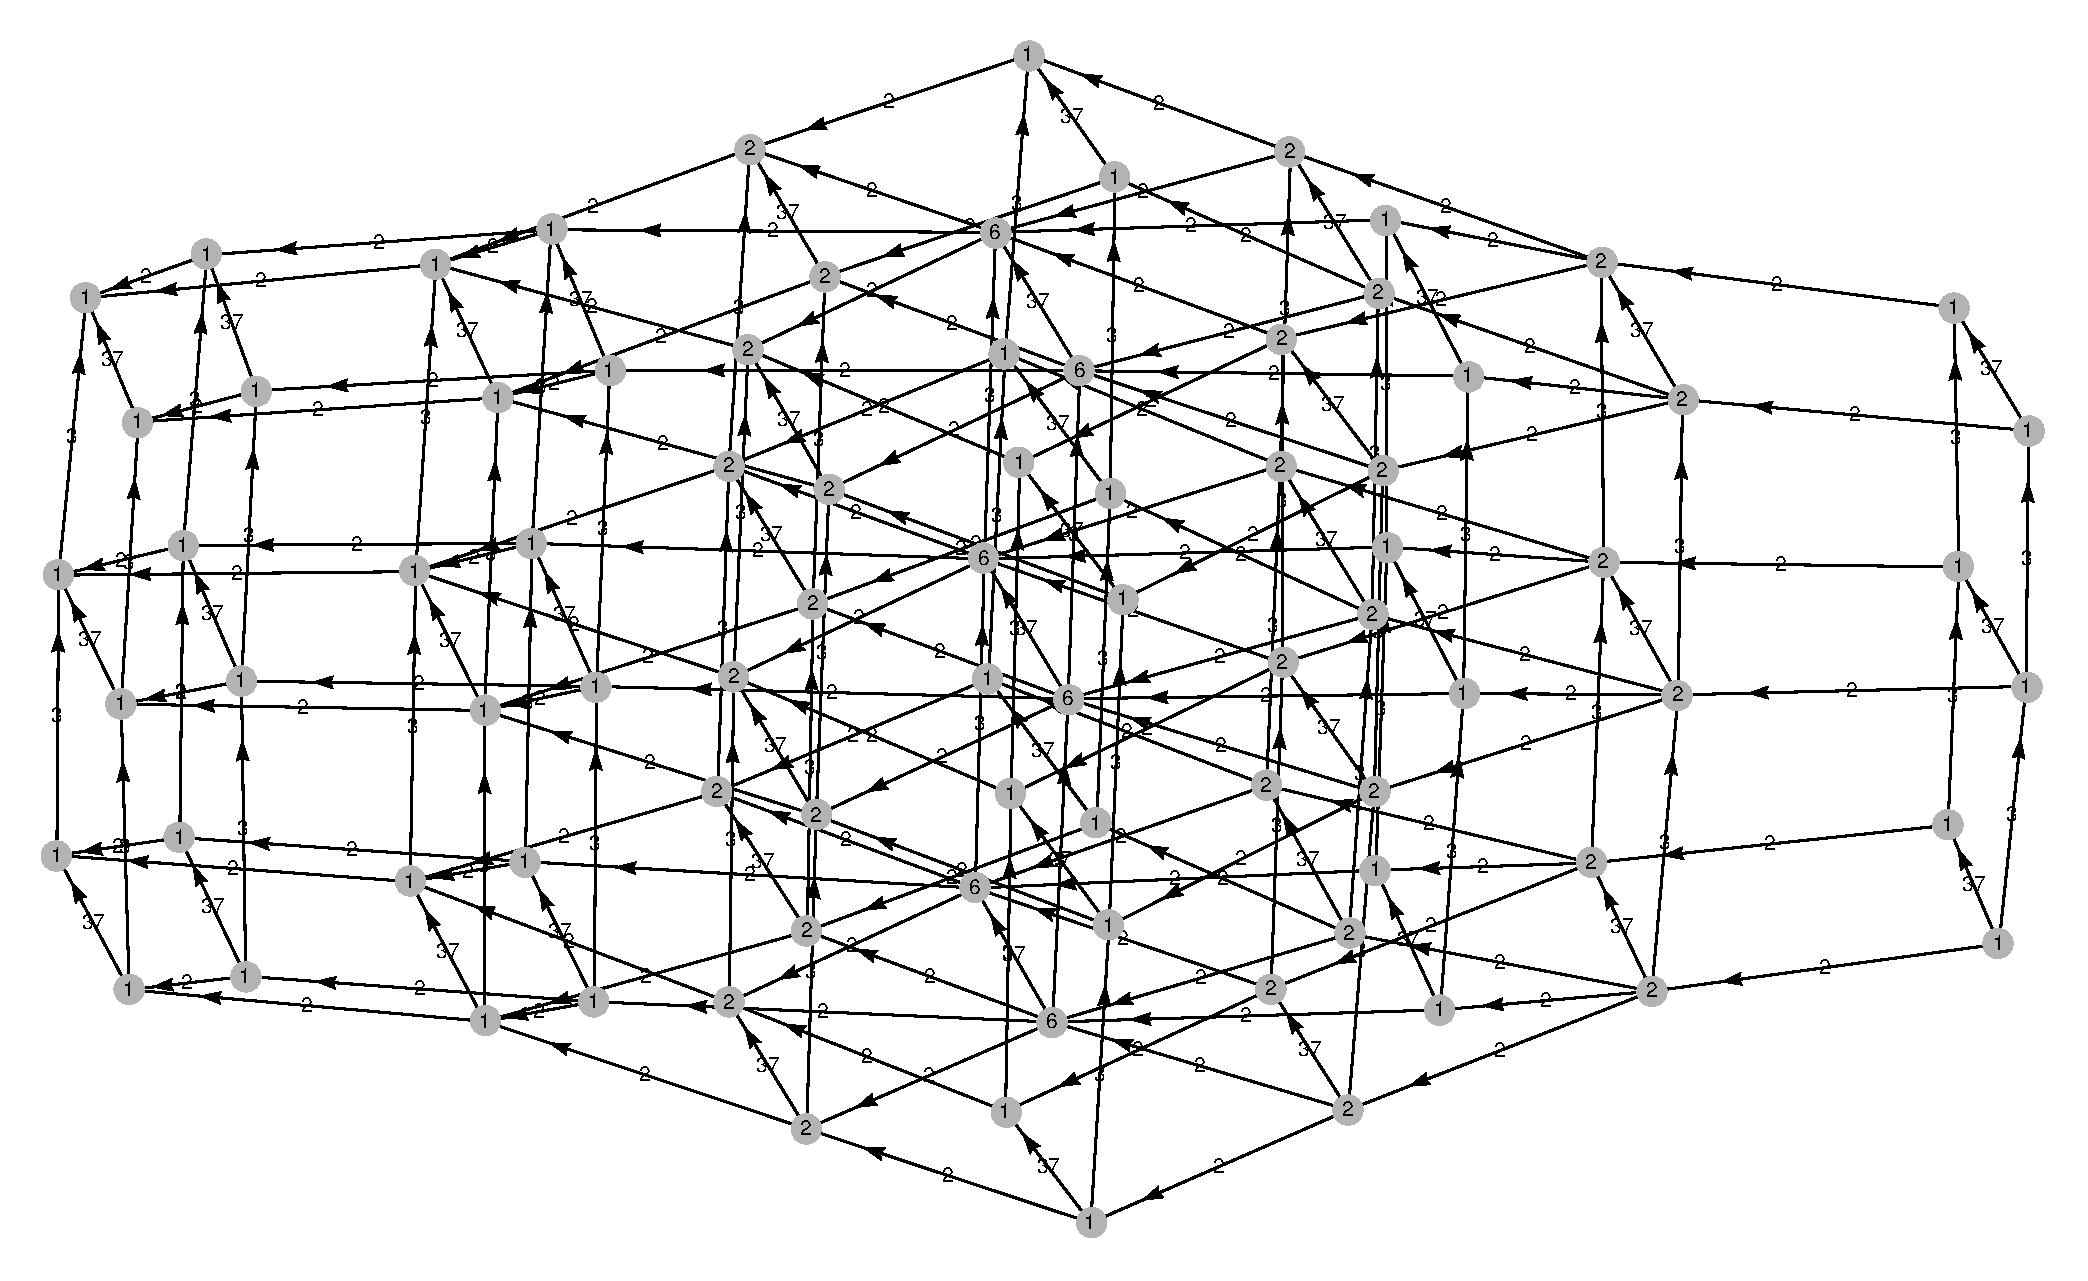
\includegraphics[width=1\textwidth]{graph-1}
% \end{figure}
% \vspace{-2 em} Weak equivalence classes of the monogenic order of $\Q[x]/(f)$ where
% \[ f=(x^2+4x+7)(x^3−9x^2−3x−1). \] 
% \end{frame}

\begin{frame}{ back to AV's: Dual variety/Polarization }
Using Howe ('95) in the \red{ordinary} \green{square-free} case: 
\begin{theorem}[M.]
   If $A\leftrightarrow I$, then:
   \begin{itemize}
      \pause \item $A^\vee \leftrightarrow \overline{I}^t$.
      \pause \item a polarization $\mu$ of $A$ corresponds to a $\lambda\in K^\times$ such that\\
	    - $\lambda I \subseteq \overline{I}^t$ (isogeny);\\
	    - $\lambda$ is totally imaginary ($\overline \lambda = -\lambda$);\\
	    - $\lambda$ is $\Phi$-positive, where $\Phi$ is a \red{specific} CM-type of $K$. \red{Bottleneck 3}\\ 
      Also: $\deg \mu= [\overline{I}^t : \lambda I]$.
      \pause  \item if $(A,\mu) \leftrightarrow (I,\lambda)$ and $S=(I:I)$ then
     \vspace{-0.5em}
	      \[\set{\parbox[p]{7.5em}{non-isomorphic polarizations of $A$}} \longleftrightarrow \dfrac{\set{\text{totally positive }u\in S^\times }}{\set{v\overline{v}: v\in S^\times}}. \red{"Bottleneck" 4}\]
     \vspace{-1em}
	 \pause \item  and $\Aut(A,\mu) = \set{\text{torsion units of $S$}}$.
\end{itemize}
\end{theorem}
\end{frame}

%\begin{frame}{ Example}
%\begin{itemize}
% \item Let $h(x)=x^8 - 5x^7 + 13x^6 - 25x^5 + 44x^4 - 75x^3 + 117x^2 - 135x + 81$.
% \item $\rightsquigarrow$ isogeny class of an simple ordinary abelian varieties over $\F_{3}$ of dimension $4$.
% \item Let $F$ be a root of $h(x)$ and put $R:=\Z[F,3/F]\subset \Q(F)$.
% \item $8$ over-orders of $R$: two of them are not Gorenstein.
% \item $\#\ICM(R) = 18 \rightsquigarrow 18$ isom.~classes of AV in the isogeny class.
% \item $5$ are not invertible in their multiplicator ring.
% \item $8$ classes admit principal polarizations.
% \item $10$ isomorphism classes of princ. polarized AV.
%\end{itemize}
%\end{frame}
%\begin{frame}{Example}{}
%Concretely:
%{\scriptsize \begin{align*}
%  \begin{split} 
%  I_1 = & 2645633792595191 \Z \oplus (F + 836920075614551) \Z \oplus (F^2 + 1474295643839839)\Z \oplus\\
%	& \oplus (F^3 + 1372829830503387)\Z \oplus (F^4 + 1072904687510)\Z \oplus\\
%	& \oplus \frac{1}{3}(F^5 + F^4 + F^3 + 2F^2 + 2F + 6704806986143610)\Z \oplus\\
%	& \oplus \frac{1}{9}(F^6 + F^5 + F^4 + 8F^3 + 2F^2 + 2991665243621169) \Z \oplus\\
%	& \oplus \frac{1}{27}(F^7 + F^6 + F^5 + 17F^4 + 20F^3 + 9F^2 + 68015312518722201)\Z\\
%  \end{split}
%\intertext{principal polarizations:}
%  \begin{split}
%  x_{1,1} = \frac{1}{27}( & -121922F^7 + 588604F^6 - 1422437F^5 +\\
%			  & +1464239F^4 + 1196576F^3 - 7570722F^2 + 15316479F - 12821193)\\ 
%%   \end{split}\\
%%   \begin{split}
%  x_{1,2} = \frac{1}{27}( & 3015467F^7 - 17689816F^6 + 35965592F^5 -\\
%			  & -64660346F^4 + 121230619F^3 - 191117052F^2 + 315021546F - 300025458)\\
%  \end{split}\\
%  & \End(I_1) =  R\\
%  & \#\Aut(I_1,x_{1,1}) = \#\Aut(I_1,x_{1,2}) = 2
% \end{align*}}
%\end{frame}
%
%
%\begin{frame}{Example}
% 
%{\scriptsize \begin{align*}
%  \begin{split} 
%  I_7 = & 2\Z\oplus(F + 1)\Z\oplus(F^2 + 1)\Z\oplus(F^3 + 1)\Z\oplus(F^4 + 1)\Z\oplus\frac13(F^5 + F^4 + F^3 + 2F^2 + 2F + 3)\Z \oplus \\ 		      & \oplus\frac{1}{36}(F^6 + F^5 + 10F^4 + 26F^3 + 2F^2 + 27F + 45)\Z\oplus\\
%	& \oplus \frac{1}{216}(F^7 + 4F^6 + 49F^5 + 200F^4 + 116F^3 + 105F^2 + 198F + 351)\Z\\
%  \end{split}
%\intertext{principal polarization:}\\[-7ex]
%  \begin{split}
%  x_{7,1} = \frac{1}{54}(20F^7 - 43F^6 + 155F^5 - 308F^4 + 580F^3 - 1116F^2 + 2205F - 1809)
%  \end{split}\\
%  \begin{split}
%  \End(I_7) & = \Z \oplus  F\Z \oplus  F^2\Z \oplus  F^3\Z \oplus  F^4\Z \oplus
%  \frac{1}{3}(F^5 + F^4 + F^3 + 2F^2 + 2F)\Z \oplus \\
%	& \oplus \frac{1}{18}(F^6 + F^5 + 10F^4 + 8F^3 + 2F^2 + 9F + 9)\Z \oplus\\
%	& \oplus \frac{1}{108}(F^7 + 4F^6 + 13F^5 + 56F^4 + 80F^3 + 33F^2 + 18F + 27)\Z\\
%  \end{split}\\
%  & \#\Aut(I_7,x_{7,1}) = 2
%\end{align*}}             
%$I_1$ is invertible in $R$, but $I_7$ is not invertible in $\End(I_7)$.
%\end{frame}

\begin{frame}{Work in progress and Bottlenecks}{}
    Work in progress
	\begin{itemize}
	\item 1: polarizations in the non-ordinary (Centeleghe-Stix) square-free case (with Jonas Bergstr\"om)
	\item 2: group of rational points (and level structure)
% 	\item 3: polarizations in the $E^3$ case (with Christophe Ritenthaler)
	\end{itemize}
	\pause 
	Bottlenecks
	\begin{itemize}
	\item 1: over-orders (Tommy Hoffman ?)
	\item 2: weak equivalence class monoid (I have a conjecture)
	\item 3: CM-type (need to compute a splitting field. can be done locally?)
	\item 4: polarizations (it should be possible to "spread" them)
	\end{itemize}
\end{frame}

%\begin{frame}{some results from computations}{}
%   {\footnotesize
%   \begin{tabular}{| c | c | c | c | c | c | c |}
%   \hline
% 		& isogeny cl.     & isom.cl.     & \parbox{3.6 em}{isom.cl.\\no p.pol.} & \parbox{3.7 em}{isom.cl.\\w/p.pol.} & \parbox{3.3 em}{isom.w/\\${\End=\cO_K}$} & \parbox{3.6 em}{isom.cl.\\no p.pol.\\${\End=\cO_K}$}\\\hline
%      $\F_2,g=2$ & $14/34$         & $21$	  & $7$ 	       & $15$	& $15$	& $3$ \\\hline     
%      $\F_3,g=2$ & $36/62$         & $76$	  & $23$ 	       & $59$	& $43$	& $6$\\\hline
%      $\F_5,g=2$ & $94/128$        & $457$	  & $207$ 	       & $286$	& $159$	& $34$\\\hline
%      $\F_7,g=2$ & $168/207$       & $1324$  	  & $638$ 	       & $795$	& $387$	& $88$\\\hline
%      $\F_{11},g=2$ & $352/400$    & $4925$  	  & $2675$ 	       & $2797$	& $1476$& $459$\\\hline
%      $\F_2,g=3$ & $82/210$        & $226$	  & $102$ 	       & $142$	& $112$	& $16$\\\hline
% \red{$\F_3,g=3$}& $366/670$	  & $2508$  	  & $1287$	       & $1492$	& $874$	& $187$\\\hline     
% \red{$\F_5,g=3$}& $439/2994$	  & $30867$	  & $24693$ 	       & $7013$	& $836$	& $206$\\\hline     
% \red{$\F_7,g=3$}& $267/7968$	  & $26506$  	  & $21557$ 	       & $5674$	& $721$	& $180$\\\hline     
% \red{$\F_{11},g=3$}& $188/30530$  & $18513$ & $14291$	       & $4830$	& $614$	& $150$\\\hline
%   \end{tabular}
%   }\vspace{1 em}
% 
%   black = all ordinary squarefree isogeny classes have been computed
%   
%   \red{red = work in progress}
%\end{frame}

% \begin{frame}{ Final remarks }
% \begin{itemize}
% %    \item the same correspondence between iso.~classes of AV's and $\ICM$ holds for isogeny classes $\cC_h$ over $\F_p$ with $h(\sqrt{p})\neq 0$ square-free\\
% % \pause much larger subcategory ... but no polarizations in this case.
% % 	  (Centeleghe and Stix 2015)
%          \item Using Centeleghe-Stix '15 we can compute the isomorphism classes in $\cC_h$ over $\F_p$  where $h$ is \textbf{square-free} and \textbf{without real roots}.\\
% \pause much larger subcategory!!! ... but no polarizations in this case.         
% \pause   \item we can also deal with the case $\cC_{h^d}$ (with $h$ square-free) when $\Z[F,q/F]$ is Bass (soon on arXiv).
% \pause   \item base field extensions (ordinary case).
% \pause   \item period matrices (ordinary case) of the canonical lift.
% % \pause   \item conjugacy classes of integral matrices.
% \end{itemize}
% \end{frame}

%\begin{frame}{ }
%\begin{center}
%{\Large Thank you!}
%\end{center}
%\end{frame}

\end{document}
